\chapter{2D Systems}\label{ch:2Dsyst}
Can be used to model drum membranes, plate reverbs or simplified instrument bodies (as done in this work). 

First the 2D wave equation, the 2D-equivalent of the 1D wave equation presented in Section \ref{sec:1DWave} will be presented. The model, some of the differences between the analysis techniques presented in Chapter \ref{ch:analysis} and those in 2D will be elaborated on.\footnote{The abbreviation 2D will also be used for `two dimensions'.}

The systems modelled in this work are simplified to be rectangular and are defined on a Cartesian coordinate system. Section \ref{sec:radialCoordinates} briefly elaborates on radial coordinate systems and their shortcomings. 



Unless denoted otherwise, the theory in this chapter follows \cite{theBible}.

\section{PDEs and FD schemes in 2D}
Consider a rectangular 2D system with side lengths $L_x$ and $L_y$ (both in m) and its state described by $u = u(x,y,t)$. The system is defined for $t\geq 0$ and $(x,y) \in \D$ where domain $\D \in [0, L_x]\times [0, L_y]$ is two-dimensional. 

Similar to the 1D case in Section \ref{sec:gridFunctions}, state variable can be discretised to a 2D grid function according to $u(x, y, t) \approxeq \ulmn$ with space $x = lh$ and $y = mh$ and time $t = nk$ and $k=1/\fs$. For simplicity, in this work the grid spacing $h$ is set to be the same in both the $x$ and $y$ directions.

\subsubsection{Additional operators}
In continuous time, an additional operator, referred to as the \textit{Laplacian} can be defined as
\begin{equation}\label{eq:laplacian}
    \Delta = \pxx + \pyy,
\end{equation}
which describes a second-order spatial derivative in 2D. A fourth-order spatial derivative in 2D, used to model stiffness in a system is called the \textit{biharmonic} operator and is the Laplacian in Eq. \eqref{eq:laplacian} applied to itself:
\begin{equation}\label{eq:biharmonic}
    \Delta\Delta = \pxxxx + 2\pxx\pyy +  \partial_y^4,
\end{equation}

In discrete time, the same temporal and spatial shift operators as defined in Section \ref{sec:FDoperators} can be applied to grid function $\ulmn$ the latter of which only affects the spatial index $l$. Additional operators affecting spatial index $m$ for the $y$ direction are
\begin{equation}
    e_{y+}\ulmn = u_{l, m+1}^n,\quad \text{and}\quad e_{y-}\ulmn= u_{l, m-1}^n.
\end{equation}
Using these shift operators, a discrete approximation of the Laplacian in Eq. \eqref{eq:laplacian} can be made\footnote{Notice that the $\dDelta$ operator is identical to the $\delta_{\Delta \boxplus}$ in \cite{theBible}, but not used here as Eq. \eqref{eq:discreteLaplacian} is the only discretisation to the $\Delta$ operator used in this work.} 
\begin{equation}\label{eq:discreteLaplacian}
    \Delta \approxeq \dDelta \triangleq \frac{1}{h^2}\left(e_{x+} + e_{x-} + e_{y+} + e_{y-} - 4\right),
\end{equation}
and when applied to a grid function yields
\begin{equation}\label{eq:laplacianExpansion}
    \Delta u \approxeq \dDelta \ulmn = \frac{1}{h^2}\left(u_{l+1, m}^n + u_{l-1, m}^n+u_{l, m+1}^n+u_{l, m-1}^n - 4 \ulmn\right). 
\end{equation}
 Similarly an approximation of the biharmonic operator in Eq. \eqref{eq:biharmonic} can be made as
\begin{equation}\label{eq:discreteBiharmonic}
% \begin{align}
        \Delta\Delta \approxeq \dDelta\dDelta 
        % &= \begin{aligned}[t]
        %     \frac{1}{h^4}\Bigg(&\left(e_{x+}^2 + 1+ e_{x+}e_{y+} + e_{x+}e_{y-} - 4e_{x+}\right)\\
        %     & + \left(1 + e_{x-}^2 + e_{x-}e_{y+} + e_{x-}e_{y-} - 4e_{x-}\right)\\
        %     & + \left(e_{x+}e_{y+} + e_{x-}e_{y+} + e_{y+}^2 + 1 - 4e_{y+}\right)\\
        %     & + \left(e_{x+}e_{y-} + e_{x-}e_{y-} + 1 + e_{y-}^2 - 4e_{y-}\right)\\
        %     & -4 \left(e_{x+} + e_{x-} + e_{y+} + e_{y-} - 4\right)\Bigg)
        % \end{aligned}\\
        \triangleq \begin{aligned}[t]
        &\frac{1}{h^4}\bigg[\left(e_{x+}^2 + e_{x-}^2 + e_{y+}^2 + e_{y-}^2\right) \\
        &\ \ \ + 2 \left(e_{x+}e_{y+} + e_{x+}e_{y-} + e_{x-}e_{y+} + e_{x-}e_{y-}\right) \\
        &\ \ \ -8 \left(e_{x+} + e_{x-} + e_{y+} + e_{y-}\right) + 20\bigg]
    \end{aligned}
% \end{align}
\end{equation}
and when applied to a grid function yields
\begin{equation}\nonumber
    \begin{aligned}
    \Delta\Delta u\approxeq\dDelta\dDelta \ulmn =&\frac{1}{h^4}\Big[(u_{l+2, m}^n + u_{l-2, m}^n+u_{l, m+2}^n+u_{l, m-2}^n)\\
    &\ \ \ +2(u_{l+1, m+1}^n + u_{l-1, m+1}^n+u_{l+1, m-1}^n+u_{l-1, m-1}^n)\\
    &\ \ \ -8(u_{l+1, m}^n + u_{l-1, m}^n+u_{l, m+1}^n+u_{l, m-1}^n) + 20u_{l,m}^n\Big].
    \end{aligned}
\end{equation}

\section{2D Wave Equation}\label{sec:2Dwave}
The 2D wave equation be used to model an ideal membrane such as done in 

It has identical behaviour to the 2D waveguide mesh presented by van Duyne and Smith \cite{Duyne1993}.

This section will present the 2D wave equation in continuous time its discretisation afterwards. Then it will be used as a test-case to explain the various analysis techniques presented in Chapter \ref{ch:analysis} in 2D.

\subsection{Continuous time}
Consider a system modelling the 2D wave equation with side lengths $L_x$ and $L_y$ (both in m) and its state described by $u = u(x,y,t)$. The system is defined over $(x,y) \in \D$ with domain $\D = [0, L_x] \times[0, L_y]$ and its motion is described by the following PDE
\begin{equation}\label{eq:2DwavePDE}
    \ptt u = c^2\Delta u,
\end{equation}
with wave speed $c$ (in m/s) and the Laplacian operator as defined in Eq. \eqref{eq:laplacian}. If the 2D wave equation models an ideal membrane, the wave speed is defined as $c = \sqrt{T/\rho H}$, with tension per unit length (applied to the boundary)\todo{check whether this is right..} $T$ (in N/m), material density $\rho$ (in kg/m$^3$) and thickness $H$.

\subsubsection{Boundary conditions}
Similar to the 1D wave equation, two alternatives for boundary conditions are\footnote{$\forall x$ means 'for all values of $x$'.}
\begin{subequations}\label{eq:boundaryCond2DWave}
    \begin{align}
    \begin{rightcases}
        u(0, y, t) = u(L_x, y, t) = 0\quad \forall y, \\
        u(x, 0, t) = u(x, L_y, t) = 0\quad \forall x, 
    \end{rightcases}\quad &\text{(Dirichlet, fixed)},\label{eq:contDirichlet2D}\\
    \begin{rightcases}
        \px u(0, y, t) = \px u(L_x, y, t) = 0\quad \forall y,\\
        \py u(x, 0, t) = \py u(x, L_y, t) = 0\quad \forall x, 
    \end{rightcases}\quad &\text{(Neumann, free)}.\label{eq:contNeumann2D}
    \end{align}
\end{subequations}

\subsection{Discrete time}
Using the definition for the approximation of the Laplacian in Eq. \eqref{eq:discreteLaplacian}, the 2D wave equation PDE in Eq. \eqref{eq:2DwavePDE} can be discretised to
\begin{equation}\label{eq:2DwaveFDS}
    \dtt \ulmn = c^2 \dDelta \ulmn,
\end{equation}
with $l\in\{0, \hdots, N_x\}$ and $m\in \{0, \hdots, N_y\}$ where $N_x$ and $N_y$ are the number of intervals between grid points in the $x$ and $y$ direction respectively. The operators can then be expanded (see Eq. \eqref{eq:laplacianExpansion}) and solving for $\ulm^n$ yields the following update equation 
\begin{equation}\label{eq:update2Dwave}
    \ulm^{n+1} = 2\ulmn - \ulm^{n-1} + \lambda^2 \left(u_{l+1, m}^n + u_{l-1, m}^n+u_{l, m+1}^n+u_{l, m-1}^n - 4 \ulmn\right),
\end{equation}
where the Courant number 
\begin{equation}\label{eq:courant2D}
    \lambda = \frac{ck}{h},
\end{equation}
and needs to abide
\begin{equation}\label{eq:CFL2D}
    \lambda \leq \frac{1}{\sqrt{2}}
\end{equation}
for the scheme to be stable (see Section \ref{sec:stability2Dwave}). Writing this condition in terms of the grid spacing  
\begin{equation}\label{eq:stabilityCondition2Dwave}
    h \geq \sqrt{2}ck\ .
\end{equation}

\subsubsection{Discrete boundary conditions}
The continuous-time boundary conditions in Eqs. \eqref{eq:boundaryCond2DWave} can be discretised to 
\begin{subequations}\label{eq:boundaryCond2DWaveDisc}
    \begin{align}
    \begin{rightcases}
        u_{0,m}^n = u_{N_x,m}^n = 0&&\quad \forall m, \\
        u_{l,0}^n = u_{l,N_y}^n = 0&&\quad \forall l, 
    \end{rightcases}\quad &\text{(Dirichlet, fixed)},\label{eq:discDirichlet2D}\\
    \begin{rightcases}
        \dxd u_{0,m}^n = \dxd u_{N_x,m}^n = 0&&\quad \forall m, \\
        \dyd u_{l,0}^n = \dyd u_{l,N_y}^n = 0&&\quad \forall l, 
    \end{rightcases}\quad &\text{(Neumann, free)}.\label{eq:discNeumann2D}
    \end{align}
\end{subequations}
If the Dirichlet boundary conditions are used (for all sides), the domain of calculation can be reduced to $l\in\{1, \hdots N_x-1\}$ and $m\in\{1, \hdots N_y-1\}$. 

\subsubsection{Stencil}
Figure \ref{fig:stencil2Dwave} shows the stencil of the 2D wave equation FD scheme in Eq. \eqref{eq:2DwaveFDS}. Due to the extra dimension, layout of the stencil is made to account for this. The colour-coding for grid points at the various time steps is unchanged.

\begin{figure}[h]
    \centering
    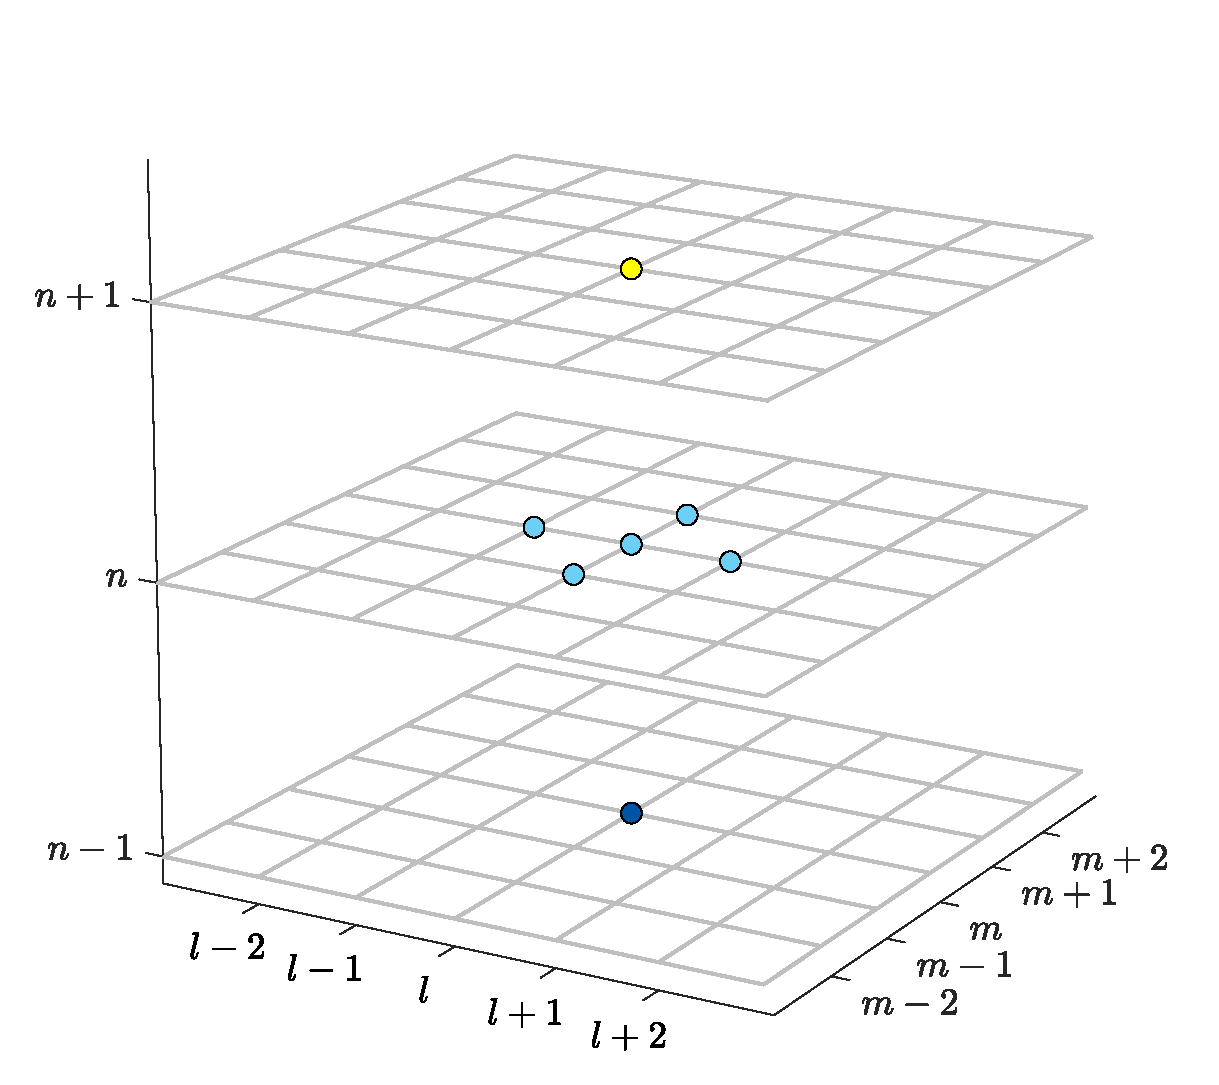
\includegraphics[width=0.7\textwidth]{figures/resonators/2d/stencil2Dwave.eps}
    \caption{The stencil for the 2D wave equation FD scheme in Eq. \eqref{eq:2DwaveFDS}. The grid points use the same colour-coding as previous stencils (see e.g. Figure \ref{fig:stencil1DWave}).\label{fig:stencil2Dwave}}
\end{figure}
\subsection{Implementation and Matrix Form}\label{sec:2DwaveImplementation}
Similar to how the number of intervals between grid points are calculated 1D in Eq. \eqref{eq:orderOfCalc}, these can be calculated using the following operations:
\begin{equation}\label{eq:orderOfCalc2D}
    h := \sqrt{2} ck, \ \ N_x := \floor[\frac{L_x}{h}], \ \  N_y := \floor[\frac{L_y}{h}], \ \  h := \text{min}\left(\frac{L_x}{N_x}, \frac{L_y}{N_y}\right), \ \  \lambda := \frac{ck}{h}.
\end{equation}
% Notice that the grid spacing is recalculated based the smallest valueof $L_x/N_x$  $L_y/N_y$ $L/N$ for in the $x$ and $y$ direction to stay as close to the stability condition in Eq. \eqref{eq:stabilityCondition2Dwave}.
To implement the update equation in Eq. \eqref{eq:update2Dwave}, one could save the states of the system in matrices (as opposed to vectors in the 1D case) and directly work with these. Using Dirichlet boundary conditions the $(N_x-1) \times (N_y-1)$ state matrix at time index $n$ will be 
\begin{equation}
    \u^n = \begin{bmatrix}
        u^n_{1, 1} & \hdots & u^n_{1, N_x-1}\\
        \vdots & \ddots & \vdots\\
        u^n_{N_y-1, 1} & \hdots & u^n_{N_y-1, N_x-1}
    \end{bmatrix}
\end{equation}

This matrix can then be used to make a `for-loop implementation' of the update equation, which would be the strategy if the scheme would be implemented in C++ (see Chapter \ref{ch:realtime}). For a more compact implementation in \texttt{MATLAB}, one could `stack' the state matrices to vectors (see Figure \ref{fig:stackingMatrix}) and update the scheme using matrix-vector multiplication as done for, e.g., the stiff string in Section \ref{sec:implementationStiffString}. Again using Dirichlet boundary conditions, the stacked state vector of size will be structured as
\begin{equation}
    \U^n = [(\u_{1}^n)^T, \hdots, (\u_{N_x-1}^n)^T]^T, \qwiq \u^n_l = [u^n_{l, 1}, \hdots, u^n_{l, N_y-1}]^T,
\end{equation}
and has a size of $(N_x-1)\cdot (N_y-1) \times 1$.

To create a matrix form of the $\dDelta$ operator, the \textit{kronecker product} and \textit{kronecker sum} must be introduced \cite{Horn1991}. The kronecker product between two arbitrarily-sized matrices (using their dimensions as a subscript) is
\begin{equation}
    \A_{M\times N} \otimes \B_{K\times L} = \begin{bmatrix}
        a_{11}\B & \hdots & a_{1N}\B\\
        \vdots & \ddots & \vdots\\
        a_{M1}\B & \hdots & a_{MN}\B\\
    \end{bmatrix}_{MK \times NL}.
\end{equation}
% In essence, the kronecker product copies a matrix $\B$ according to a matrix $\A$. gets arranged according to a 
% The matrix operators then use the kronecker
The kronecker sum between two square matrices is 
\begin{equation}
    \A_{M \times M} \oplus \B_{N \times N} = \I_N\otimes \A + \B \otimes\I_M,
\end{equation}
where $\I_P$ is the identity matrix of size $P\times P$. 

For Dirichlet boundary conditions, the $\Dxx$ matrix of size $(N_x-1) \times (N_x-1)$ and the $\Dyy$ matrix of size $(N_y-1) \times (N_y-1)$ can be defined (similarly to Eq. \eqref{eq:DxxDef}) as
%
\setstackgap{L}{14pt}
\setstacktabbedgap{3pt}
\def\lrgap{\kern3pt}
\fixTABwidth{T}
%
\begin{equation}\label{eq:DxxyyDef}
    \Dxx = \frac{1}{h^2}\underbrace{\xbracketMatrixstack{
        -2 & 1 & & &\mathbf{0}\\
        1 & -2 & 1 & & \\
        & \ddots & \ddots & \ddots & \\
        & & 1 & -2 & 1 \\
        \mathbf{0}& & & 1 & -2 
    }}_{(N_x-1) \times (N_x-1)} \qaq \Dyy = \frac{1}{h^2}\underbrace{\xbracketMatrixstack{
        -2 & 1 & & &\mathbf{0}\\
        1 & -2 & 1 & & \\
        & \ddots & \ddots & \ddots & \\
        & & 1 & -2 & 1 \\
        \mathbf{0}& & & 1 & -2 
    }}_{(N_y-1) \times (N_y-1)}
\end{equation}
%
Following \cite{Hamilton2016}, the matrix form of the $\dDelta$ operator can then be defined as the kronecker sum of $\Dyy$ and $\Dxx$ yielding
%
\setstackgap{L}{14pt}
\setstacktabbedgap{2pt}
\def\lrgap{\kern3pt}
\fixTABwidth{T}
%
\begin{equation}
    \DDeltamat = \Dyy \oplus \Dxx = \xbracketMatrixstack{
        \ddots & & & & \mathbf{0}\\
        &\Dyy & & & \\
        & &\Dyy & & \\
        & & & \Dyy & \\
        \mathbf{0}& & & & \ddots
    } + \frac{1}{h^2}\!\!\xbracketMatrixstack{
         \ddots&\ddots & & & \mathbf{0}\\
         \ddots&-2\I&\I & & \\
        &\I&-2\I &\I &  \\
        & & \I& -2\I &\ddots\\
        \mathbf{0}& & & \ddots& \ddots
    }
\end{equation}
where the identity matrix $\I = \I_{N_x-1}$. The $\DDeltamat$ matrix is square and of size $(N_x-1)\cdot (N_y-1)\times (N_x-1)\cdot (N_y-1)$.
\begin{figure}[t]
    \centering
    \includegraphics[width=\textwidth]{figures/resonators/2d/stackingMatrix.pdf}
    \caption{Stacking, or `flattening' a $4\times 4$ matrix to a $16$-element vector. \label{fig:stackingMatrix}}
\end{figure}
Using the above, the update equation in Eq. \eqref{eq:update2Dwave} can then be compactly written in matrix form as
\begin{equation}\label{eq:matrixUpdate2Dwave}
    \U^{n+1} = \left(2 \I + c^2k^2 \DDeltamat\right) \U^n - \U^{n-1},
\end{equation}
where the identity matrix is of the same size as $\DDeltamat$. See Appendix \ref{app:2DWave} for an implementation of the 2D wave equation using the update equation in Eq. \eqref{eq:matrixUpdate2Dwave}.

If one would like to visualise the system state as a 2D grid, one can revert the stacked vector back to a matrix by using the \texttt{reshape} function in \texttt{MATLAB}:
\begin{center}
    \texttt{uMatrix = reshape(u, Ny-1, Nx-1);}
\end{center}
A 2D raised-cosine excitation can be implemented in the same way by reshaping an excitation matrix to a vector (see lines 40--52 in Appendix \ref{app:2DWave})\todo{check if this is still true}.

\subsubsection{Output}
\SWcomment[still need to write and add figures and such]

\subsection{Frequency Domain Analysis in 2D}\label{sec:stability2Dwave}
Section \ref{sec:stabilityAnalysis} showed how to perform frequency domain analysis on an FD scheme to obtain stability conditions. This section shows extensions to this in 2D and follows \cite[Ch. 10]{theBible}.

In 2D the ansatz in Eq. \eqref{eq:ansatz} is extended to 
\begin{equation}
    \ulmn = z^n e^{jh(l\beta_x + m\beta_y)}
\end{equation}
where $\beta_x$ and $\beta_y$ are components of a 2D wavenumber $\boldsymbol{\beta}$ in the $x$ and $y$ directions respectively. Frequency-domain representations of temporal operators shown in Eq. \eqref{eq:temporalAnsatz} do not change in the 2D case. Using 
\begin{equation}\label{eq:pxpy}
    p_x = \sin^2(\beta_x h/2) \qaq p_y = \sin^2(\beta_y h/2)
\end{equation}
for brevity, the following frequency-domain representation of spatial operators can be obtained
\begin{equation}
    \dxx \ulmn \ansatz -\frac{4}{h^2}p_x 
    \ulmn \qaq \dyy \ulmn \ansatz -\frac{4}{h^2}p_y 
    \ulmn,
\end{equation}
from which it follows that
\begin{gather}
    \dDelta\ulmn \ansatz -\frac{4}{h^2}(p_x + p_y)\ulmn,\label{eq:laplacianAnsatz}\\
    \dDelta\dDelta\ulmn \ansatz \frac{16}{h^4}(p_x + p_y)^2\ulmn.\label{eq:biharmonicAnsatz}
\end{gather}

Using these definitions and Eq. \eqref{eq:temporalAnsatz}, a frequency-domain interpretation of the 2D wave FD scheme in Eq. \eqref{eq:2DwaveFDS} can be obtained
\begin{equation*}
    \frac{1}{k^2}\left(z - 2 +z^{-1}\right) = -\frac{4c^2}{h^2} (p_x + p_y).
\end{equation*}
Recalling Eq. \eqref{eq:courant2D}, this can be rewritten to the following characteristic equation
\begin{equation}
    z + \left(4\lambda^2(p_x + p_y)-2\right) +z^{-1} = 0.
\end{equation}
As (after multiplication by $z$) the characteristic equation is of the form in Eq. \eqref{eq:polynomialForm} and $a^{(2)} = 1$ , its roots are bounded by condition \eqref{eq:simplerCondition215} 
\begin{equation*}
    \left|4\lambda^2(p_x + p_y)-2\right| \leq 2.
\end{equation*}
Further derivation yields
\begin{align*}
    -2 &\leq 4\lambda^2(p_x + p_y)-2 \leq 2, \\
    0 &\leq 4\lambda^2(p_x + p_y) \leq 4,
\end{align*} 
and as middle term is non-negative the first condition is always satisfied, yields
\begin{equation*}
    \lambda^2(p_x + p_y) \leq 1.
\end{equation*}
Finally, as $p_x$ and $p_y$ are bounded by 1 for all wavenumbers $\beta_x$ and $\beta_y$ respectively, the following condition must hold
\begin{align}
    2\lambda^2&\leq 1,\nonumber\\
    \lambda &\leq \frac{1}{\sqrt{2}}
\end{align}
which is the stability condition given in Eq. \eqref{eq:CFL2D}.

\subsection{Energy Analysis in 2D}\label{sec:energyAnalysis2DWave}
\def\domXred{\underline{d_x}}
\def\domYred{\underline{d_y}}
\def\domXredBoth{\underline{\overline{d_x}}}
\def\domYredBoth{\underline{\overline{d_y}}}

Energy analysis for the 1D case is introduced in Section \ref{sec:energyAnalysis}. Extensions for the analysis in 2D will be given here.

Analogous to the 1D inner product presented in Section \ref{sec:innerProduct}, one can define a 2D inner product. For two functions $f = f(x,y,t)$ and $g(x,y,t)$ defined for a 2D domain $\D$ their inner product over this domain is defined as
\begin{equation}
    \langle f, g \rangle_\D  = \iint_\D f g dx dy
\end{equation}
As in the 1D case, these functions do not have to be a function of time, but are for coherence. 

For two (grid) functions $f_{l,m}^n$ and $g_{l,m}^n$ defined over a discrete domain $d\in \{0, \hdots, N_x\} \times \{0, \hdots, N_y\}$ their discrete inner product is defined as
\begin{equation}\label{eq:2DInnerProd}
    \langle f^n_{l, m}, g^n_{l, m} \rangle_d = \sum_{l = 0}^{N_x}\sum_{m = 0}^{N_y} h^2 f_{l,m}^n g_{l,m}^n.
\end{equation}
Notice that the multiplication with the grid spacing is squared due to the inner product over a 2D domain (and is the discrete counterpart of $dxdy$). Useful for energy analysis are the following reduced 2D domains 
\begin{equation}\label{eq:reduced2Ddoms}
    \begin{aligned}
        \domXred &= \{0, \hdots, N_x-1\} \times \{0, \hdots, N_y\}, \\
        \domXredBoth &= \{1, \hdots, N_x-1\} \times \{0, \hdots, N_y\},\\
        \domYred &= \{0, \hdots, N_x\} \times \{0, \hdots, N_y-1\},\\
        \domYredBoth &= \{0, \hdots, N_x\} \times \{1, \hdots, N_y-1\}
    \end{aligned}  
\end{equation}


% $\underline{d} = \{0, \hdots, N_x-1\} \times \{0, \hdots, N_y-1\}$ and $\underline{\overline{d}} = \{1, \hdots, N_x-1\}\times\{1, \hdots, N_y-1\}$.

Below, the steps to perform energy analysis presented in Section \ref{sec:energyAnalysis} will be followed:
\subsubsection{Step 1: Obtain $\dtp \h$}
Using the definition of wave speed for the ideal membrane, i.e., $c = \sqrt{T/ \rho H}$, FD scheme \eqref{eq:2DwaveFDS} can be multiplied by $\rho A$ and a 2D inner product (see Eq. \eqref{eq:2DInnerProd}) with $(\dtd \ulmn)$ over discrete domain $d$ can be taken to yield a definition for $\dtp \h$:
\begin{equation*}
    \dtp \h = \rho H\langle \dtd \ulmn , \dtt \ulmn\rangle_d - T \langle \dtd\ulmn, \dDelta \ulmn\rangle_d = 0,
\end{equation*}
which can be rewritten to
\begin{equation*}
    \dtp \h= \rho H\langle \dtd \ulmn , \dtt \ulmn\rangle_d - T \left(\langle \dtd\ulmn, \dxx \ulmn\rangle_d + \langle \dtd\ulmn, \dyy \ulmn\rangle_d \right) = 0.
\end{equation*}\todo{FULL DOC SWEEP: check what equations have numbers when performing energy analysis (and stability for that matter)}

\subsubsection{Step 2: Identify energy types and isolate $\dtp$}
Summation by parts as described in Section \ref{sec:summationByParts} can also be applied to $\dyy$ the following energy balance follows 
\begin{equation*}
    \dtp \h = \b,
\end{equation*}
where 
\begin{equation}\label{eq:energyBalance2DWave}
    \begin{gathered}
        \h = \t + \v \qwiq \t = \frac{\rho H}{2}\lVert \dtm \ulmn\rVert^2_d \quad \text{and}
        \\
        \v = \frac{T}{2} \left(\langle \dxp \ulmn, e_{t-}\dxp \ulmn\rangle_{\domXred} + \langle \dyp \ulmn, e_{t-}\dyp \ulmn\rangle_{\domYred} \right).
    \end{gathered}
\end{equation}
The boundary term is 
\begin{equation*}
    \begin{aligned}
    \b =\frac{T}{2}\Bigg[&\Big(\langle \dtd u_{N_x,m}^n, \dxp u_{N_x,m}^n \rangle_{(N_x, y)} + \langle \dtd u_{l,N_y}^n, \dyp u_{l,N_y}^n \rangle_{(x, N_y)} \Big)\\
    &-\Big(\langle \dtd u_{0,m}^n, \dxm u_{0,m}^n \rangle_{(0, y)} + \langle \dtd u_{l,0}^n, \dym u_{l,0}^n \rangle_{(x, 0)} \Big)\Bigg]\ ,
    \end{aligned}
\end{equation*}
and uses 1D inner products at the boundaries. $(l,y)$ is an inner product over a   used for the inner products  
Here, the reduced domains $\domXred$ and $\domYred$ are as defined in \eqref{eq:reduced2Ddoms}. The 

which vanish under Dirichlet boundary conditions in Eq. \eqref{eq:discDirichlet2D}.

\subsubsection{Step 3: Check units}
As the addition of the two inner products in the definition for $\v$ in Eq. \eqref{eq:energyBalance2DWave} does not affect the units, only one is used to check the units. Recalling that as opposed to the 1D case, the symbol $T$ is tension per unit length and thus in in N/m, one can write the terms in Eq. \eqref{eq:energyBalance2DWave} in their units:
\begin{align*}
    \frac{\rho H}{2}\lVert \dtm \ulmn\rVert^2_d \
    \overset{\text{in units}}{\xrightarrow{\hspace*{1cm}}}    \quad&\text{kg}\cdot\text{m}^{-3}\cdot\text{m}\cdot\text{m}^2\cdot(\text{s}^{-1}\cdot\text{m})^2 \\
    = \ & \text{kg}\cdot\text{m}^2\cdot\text{s}^{-2}\\
    \frac{T}{2} \left(\langle \dxp \ulmn, e_{t-}\dxp \ulmn\rangle_{\domXred} \right) \
    \overset{\text{in units}}{\xrightarrow{\hspace*{1cm}}}    \quad& \text{N} \cdot \text{m}^{-1}\cdot\text{m}^2\cdot(\text{m}^{-1}\cdot\text{m})\cdot(\text{m}^{-1}\cdot\text{m})\nonumber \\
    = \ &\text{kg}\cdot\text{m}^2\cdot\text{s}^{-2}
\end{align*}
which have the correct units. 

\subsubsection{Step 4: Implementation}
Figure \ref{fig:energy2Dwave} shows the energetic output of an implementation of the 2D wave equation and shows that the energy deviation is within machine precision.

\begin{figure}[h]
    \centering
    \begin{tikzpicture}[->,node distance=3cm,
        thick,main node/.style={circle,draw}]
    
        \node[] (image) at (0,0) {
        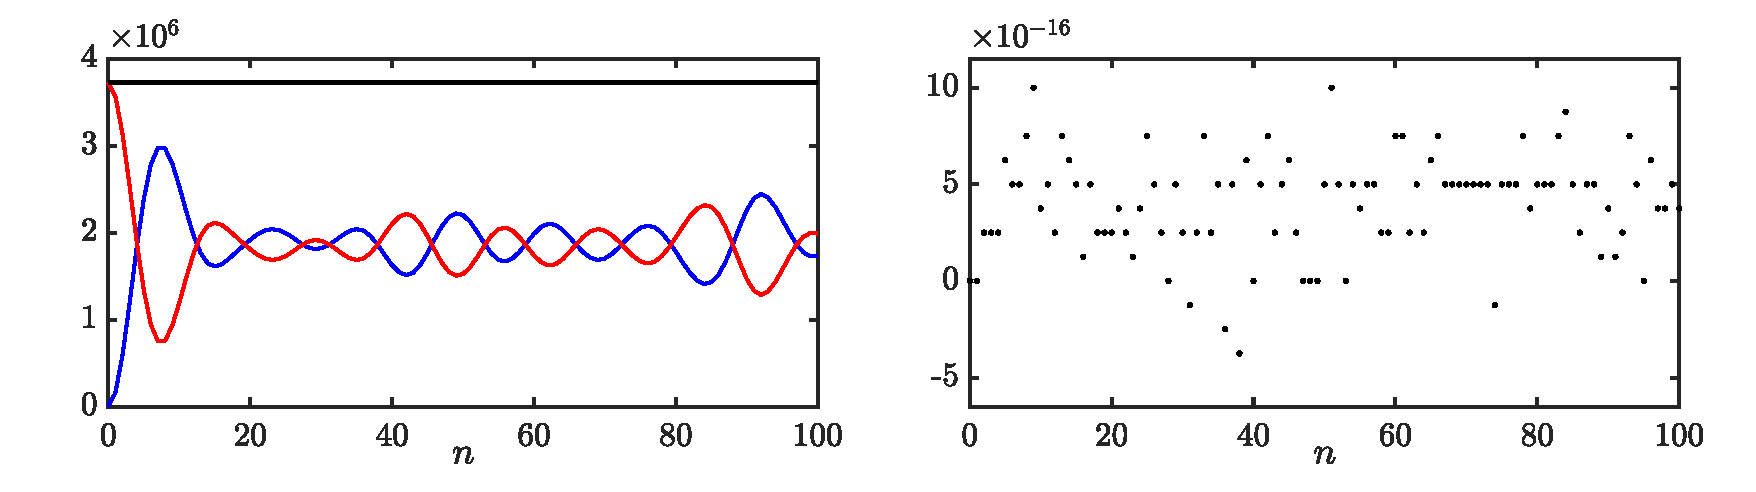
\includegraphics[width=\textwidth]{figures/resonators/2d/energy2DWave.eps}
        };
    
        \node[] (he) at (0.2,0.5) {\small $\mathfrak{h}_\text{e}$};

        \node[] (h) at (-5.75, 1) {\small $\mathfrak{h}$};
        \node[] (v) at (-5.75, 0.5) {\small $\color{red}\mathfrak{v}$};
        \node[] (t) at (-5.75, 0) {\small $\color{blue}\mathfrak{t}$};
      \end{tikzpicture}
      \caption{The kinetic (blue), potential (red), and total (black) energy of an implementation of the 2D wave equation are plotted in the left panel. The right panel shows the normalised energy (according to Eq. \eqref{eq:normalisedEnergy}) and shows that the deviation of the energy is within machine precision. \label{fig:energy2Dwave}}
\end{figure}

\subsection{Modal Analysis}
Performing a modal analysis on a 2D system does not differ from a 1D system and follows the same process presented in Section \ref{sec:modalAnalysis}, given that the state vector is stacked as described Section \ref{sec:2DwaveImplementation} and the update equation is written in matrix form as in Eq. \eqref{eq:matrixUpdate2Dwave}.

Inserting a test solution of $\U^n = z^n\boldPhi$ and following the the same process yields the following characteristic equation
\begin{equation}
   \left(z - 2 + z^{-1}\right)\boldPhi = c^2k^2\DDeltamat\boldPhi.
\end{equation}
The $p$\th modal frequency can then be obtained by finding the roots of 
\begin{equation}
    z_p + \left(-2 - c^2k^2\DDeltamat\right) + z_p^{-1} = 0,
\end{equation}
which, using test solution $z_p = e^{j\omega_p k}$ for (angular) frequency $\omega_p$, can be shown to be 
\begin{equation}\label{eq:2DWaveModes}
    f_p = \frac{1}{\pi k}\sin^{-1}\left(\frac{ck}{2}\sqrt{-\text{eig}_p(\DDeltamat)}\right).
\end{equation}
This is similar to the modal frequencies of the 1D wave equation in Eq. \eqref{eq:1DWaveModes}.

\subsubsection{Modal shapes}
Using the code in Appendix \ref{sec:eigenValueProblems} and the \texttt{reshape} function, the modal shapes of the system can also be obtained. Figure \ref{fig:modalShapes2D} shows the six lowest-freuqency modes of the 2D wave equation with $L_x = 1.5$ m and $L_y = 1$ m. The mode number $(x,y)$ corresponds to the modal number in the $x$ and $y$ direction.

\begin{figure}[h]
    \centering
    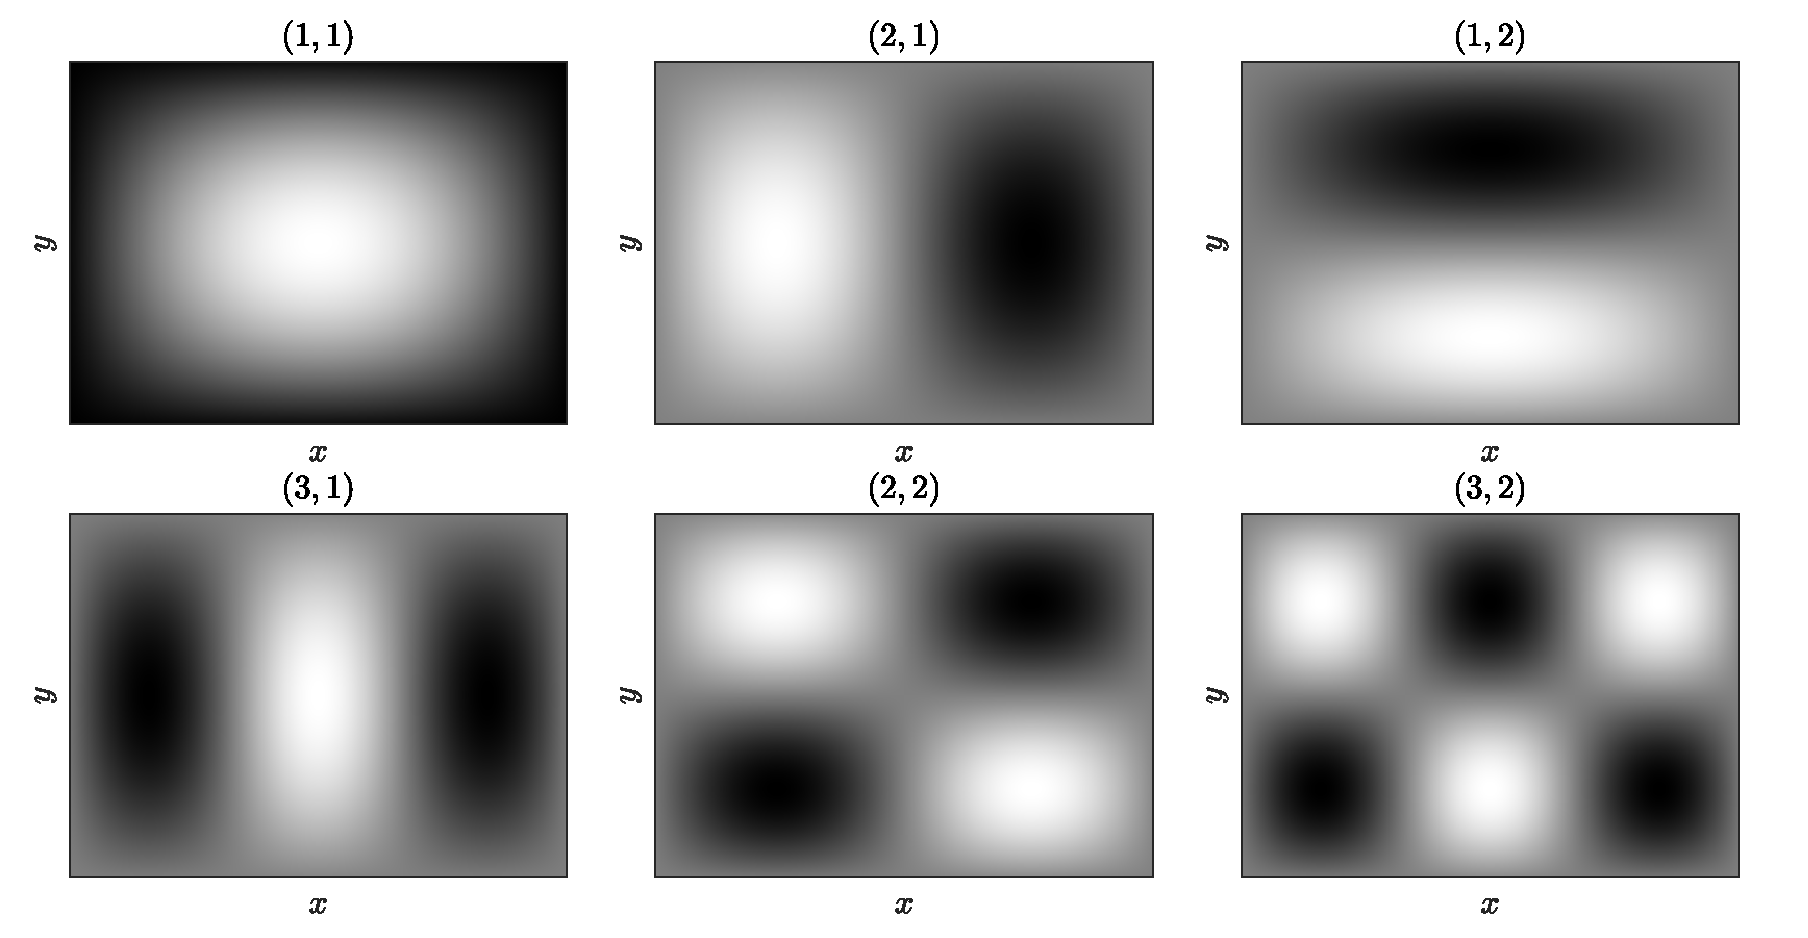
\includegraphics[width=\textwidth]{figures/resonators/2d/modalShapes.eps}
    \caption{The first (lowest-frequency) six modal shapes of 2D wave equation with $L_x = 1.5$ m and $L_y = 1$ m. \label{fig:modalShapes2D}}
\end{figure}

\section{Thin plate}\label{sec:thinPlate}
The thin plate 
Kirchoff-Love

It can be seen as the 2D extension of the ideal bar (the stiff string in Eq. \eqref{eq:stiffStringPDENoLosses} with $T=0$).

can be used to model a plate reverb \cite{DAFxChapter}


Used in \citeP[A], \citeP[B], \citeP[D] and \citeP[E] to model a simplified instrument body

\subsection{Continuous time}
Consider a rectangular thin plate with side lengths $L_x$ and $L_y$ (both in m) and its transverse displacement described by $u=u(x,y,t)$. The system is defined for $(x,y)\in \D$ where 2D domain $\D = [0, L_x]\times [0, L_y]$. Using the biharmonic operator introduced in Eq. \eqref{eq:biharmonic}, the PDE for the thin plate, also known as the Kirchhoff model, can be defined as \cite{Kirchhoff1968}
\begin{equation}\label{eq:platePDENoLosses}
    \rho H \ptt u = -D\Delta\Delta u,
\end{equation}
where $D = EH^3/12(1-\nu^2)$ is a stiffness coefficient parametrised by Young's Modulus $E$ (in Pa), thickness $H$ (in m) and the dimensionless Poisson's ratio $\nu$\todo{look up what this actually is}. Although Eq. \eqref{eq:platePDENoLosses} only holds for thin plates and only accounts for low-amplitude vibration, these properties can be assumed in musical instrument simulations making this model sufficient in this work. 

Adding losses to Eq. \eqref{eq:platePDENoLosses} yields
%
\begin{equation}\label{eq:platePDE}
    \rho H \ptt u = -D\Delta\Delta u - 2\sz \rho H \pt u + 2 \so\rho H  \pt \Delta u
\end{equation}
where, as in the case of the stiff string in Eq. \eqref{eq:stiffStringPDE}, $\sz$ and $\so$ are the frequency independent (in s$^{-1}$) and frequency dependent damping coefficient (in m$^2$/s) respectively.

\subsubsection{Boundary conditions}
Similarly to the stiff string, clamped and simply supported boundary conditions exist where
\begin{subequations}\label{eq:boundaryCondThinPlate}
    \begin{align}
        \begin{rightcases}
            u = \px u = 0\quad \text{if } y=\{0 , L_y\} \quad \forall x\\
            u = \py u = 0\quad \text{if } x=\{0 , L_x\}\quad \forall y
        \end{rightcases}
     \quad &\text{(Clamped)},\label{eq:contClamped2D}\\
     \begin{rightcases}
        u = \pxx u = 0\quad \text{if } y=\{0 , L_y\} \quad \forall x\\
        u = \pyy u = 0\quad \text{if } x=\{0 , L_x\}\quad \forall y
    \end{rightcases}\quad &\text{(Simply supported)}.\label{eq:contSimplySupported2D}
    \end{align}
\end{subequations}
 Naturally, a free condition can be added but is much less trivial. As it will not be used in this work, it will not be given here, and the interested reader is instead referred to \cite[Ch. 12]{theBible}. 

\subsection{Discrete time}
Equation \eqref{eq:platePDE} can be discretised to the following FD scheme:
\begin{equation}\label{eq:thinPlateFDS}
    \rho H \dtt \ulmn = - D \dDelta\dDelta\ulmn - 2\sz \rho H \dtd \ulmn + 2 \so \rho H \dtm \dDelta\ulmn
\end{equation}
where $l\in\{0, \hdots, N_x\}$ and $m\in\{0, \hdots, N_y\}$. Here, the backwards difference operator is used for the frequency-dependent damping term to yield an explicit scheme. A more compact way to write this scheme is after a division by $\rho H$ which yields
\begin{equation}\label{eq:thinPlateFDSCompact}
    \dtt \ulmn = - \kappa^2\dDelta\dDelta\ulmn - 2\sz\dtd \ulmn + 2 \so \dtm \dDelta\ulmn
\end{equation}
with
\begin{equation}\label{eq:kappaDef}
     \kappa = \sqrt{\frac{D}{\rho H}}.
\end{equation}
Using the expansion of the discrete biharmonic operator in Eq. \eqref{eq:discreteBiharmonic}, Eq. \eqref{eq:thinPlateFDSCompact} can be expanded and solved for $\ulm^{n+1}$ according to
\begin{equation}\label{eq:plateUpdate}
    \begin{aligned}
    \ulm^{n+1} =&(2-20\mu^2 - 4S)\ulmn \\
    &\ \ \ +(8\mu^2 + S)(u_{l+1, m}^n + u_{l-1, m}^n+u_{l, m+1}^n+u_{l, m-1}^n)\\
    &\ \ \ -2\mu^2(u_{l+1, m+1}^n + u_{l-1, m+1}^n+u_{l+1, m-1}^n+u_{l-1, m-1}^n)\\
    &\ \ \ -\mu^2(u_{l+2, m}^n + u_{l-2, m}^n+u_{l, m+2}^n+u_{l, m-2}^n),\\
    &\ \ \ + (\sz k  - 1 + 4S) \ulm^{n-1}\\
    &\ \ \ - S (u_{l+1, m}^{n-1} + u_{l-1, m}^{n-1}+u_{l, m+1}^{n-1}+u_{l, m-1}^{n-1})
    \end{aligned}
\end{equation}
where 
\begin{equation}
    \mu = \frac{\kappa k}{h^2}
\end{equation}
and $S = 2\so k / h^2$ for compactness. See Figure \ref{fig:plateStencil} for the stencil of this scheme.

The stability condition of the scheme can be shown to be
\begin{equation}\label{eq:stabilityPlate}
    h \geq 2\sqrt{k\bigg(\sigma_1^2 + \sqrt{\kappa^2+ \sigma_1^2}\bigg)},
\end{equation}
and will be derived in Section \ref{sec:stabilityThinPlate}.

\subsubsection{Discrete boundary conditions}
The boundary conditions shown in Eq. \eqref{eq:boundaryCondThinPlate} can be discretised to 
\begin{subequations}\label{eq:boundaryCondThinPlateDisc}
    \begin{align}
        \begin{rightcases}
            \begin{aligned}
                \ulmn = \dxp \ulmn = 0\quad &\text{if } m=0 \ && \forall l\\
                \ulmn = \dxm \ulmn = 0\quad &\text{if } m=N_y \ && \forall l\\
                \ulmn = \dyp \ulmn = 0\quad &\text{if } l=0 \ && \forall m\\
                \ulmn = \dym \ulmn = 0\quad &\text{if } l=N_x \ && \forall m
            \end{aligned}
        \end{rightcases}
     \quad &\text{(Clamped)},\label{eq:discClamped2D}\\
     \begin{rightcases}
        \begin{aligned}
            \ulmn = \dxx \ulmn = 0\quad &\text{if } m=\{0 , N_y\} \ &&\forall l\\
            \ulmn = \dyy \ulmn = 0\quad &\text{if } l=\{0 , N_x\}\ &&\forall m
        \end{aligned}
    \end{rightcases}\quad &\text{(Simply supported)}.\label{eq:discSimplySupported2D}
    \end{align}
\end{subequations}
The clamped condition can be implemented by simply reducing the discrete range of operation to $l = \{2, \hdots, N_x-2\}$ and $m = \{2, \hdots, N_y-2\}$. For the simply supported case, the range of operation reduces to $l = \{1, \hdots, N_x-1\}$ and $m = \{1, \hdots, N_y-1\}$. Similarly to the simply supported stiff string described in Section \ref{sec:stiffStringBoundaryConditions}, the virtual grid points needed for this condition become
\begin{align*}
    u_{-1, m}^n = -u_{1, m}^n &\qaq u_{N_x+1, m}^n = -u_{N_x-1, m}^n\quad\forall m,\\
    u_{l, -1}^n = -u_{l, -1}^n &\qaq u_{l, N_y+1}^n = -u_{l, N_y-1}^n\qquad \forall l.
\end{align*}

\subsection{Implementation and output}
If simply supported boundary conditions are considered, one can easily obtain a matrix form of the $\dDelta\dDelta$ operator by multiplying two $\DDeltamat$ operators to get $\DDeltaDelta = \DDeltamat\DDeltamat$.

Writing the scheme in matrix form yields     
\begin{equation}
    A\u^{n+1} = \B\u + \C\u^{n-1}
\end{equation}
where
\begin{gather*}
    A = (1+\sz k),\quad \B = 2\I - \kappa^2 k^2 \DDeltaDelta + 2 \so k\DDeltamat, \\
    \text{and}\quad \C = -(1-\sz k)\I - 2\so k \DDeltamat
\end{gather*}
For a much quicker implementation of the algorithm, it is useful to utilise \texttt{MATLAB}'s optimisation for sparse matrices and use the \texttt{sparse} keyword to make sparse versions of the above matrices. 

The parameters 
\begin{table}[h]
    \begin{center}
    \begin{tabular}{|l|c|c|}
        \hline
        Name & Symbol (unit) & Value\\ \hline
        Side length $x$ & $L_x$ (m) & $1$\\
        Side length $y$  & $L_y$ (m) & $1$\\
        Material density & $\rho$ (kg/m$^3$) & $7850$\\
        Thickness & $H$ (m) & $5\cdot10^{-3}$\\
        Young's modulus & $E$ (Pa) & $2\cdot10^{11}$\\
        Poisson's ratio & $\nu$ (-)& $0.3$\\
        Freq.-independent damping & $\sz$ (s$^{-1}$) & $1$\\
        Freq.-dependent damping & $\so$ (m$^2$/s) & $0.005$\\\hline
    \end{tabular}
    \caption{Parameters for the thin plate and their values most commonly used over the course of this project.\label{tab:thinPlateParams}}
    \end{center}
\end{table}
{\renewcommand{\arraystretch}{1}

\def\figSpacing{0.01\textwidth}
\def\figWidth{0.49\textwidth}
\begin{figure}[t]
    \centering
    \subfloat[Full stencil.\label{fig:fullStencilPlate}]{\includegraphics[width=\figWidth]{figures/resonators/2d/fullPlate.eps}}\\
    \subfloat[Stencil of $u_{l,m}^n$. \label{fig:curStencilPlate}]{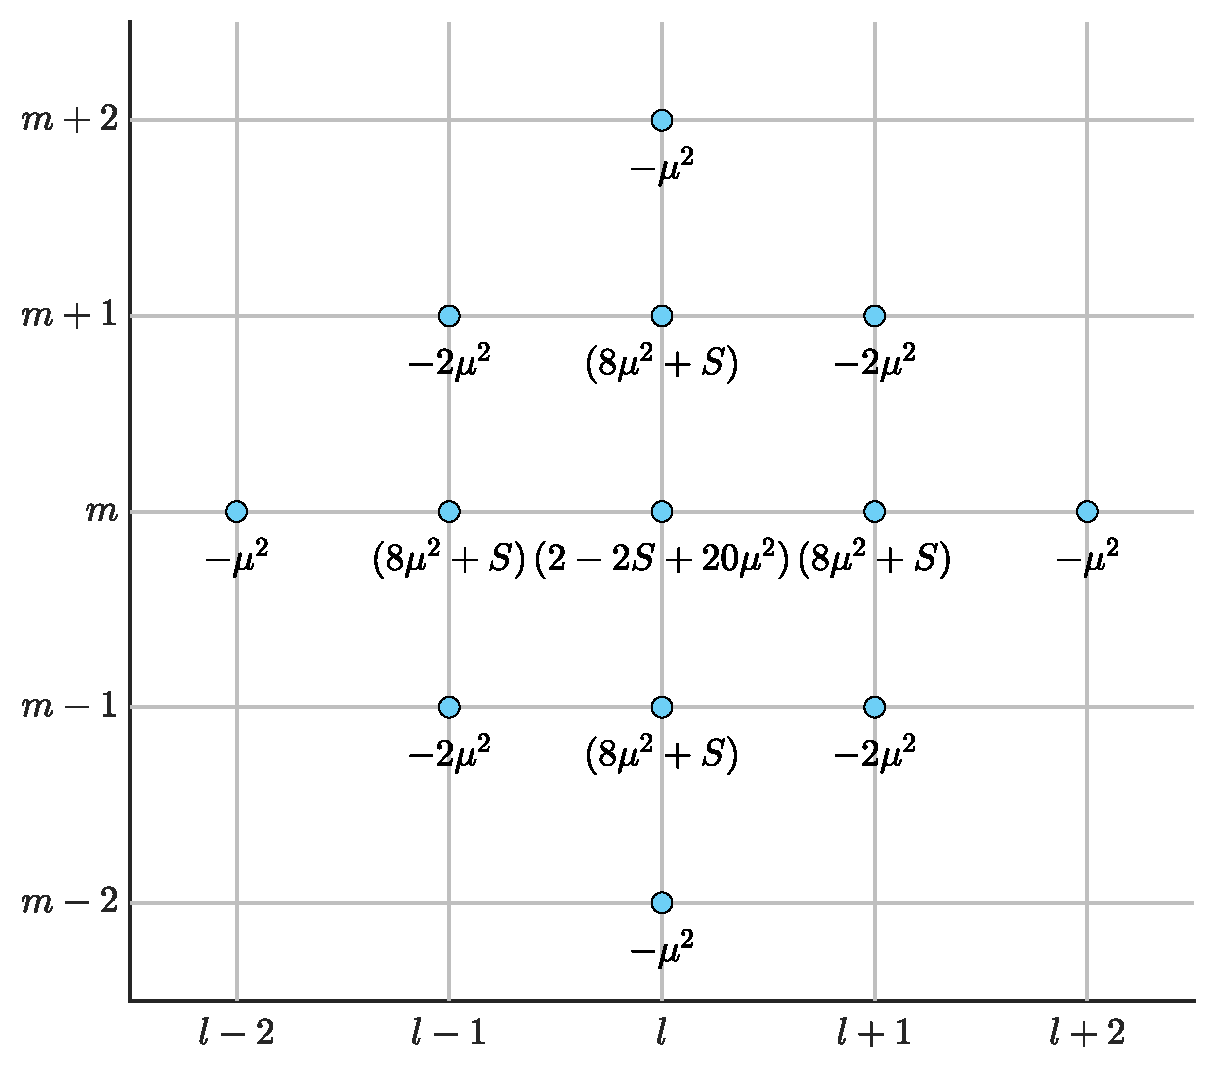
\includegraphics[width=\figWidth]{figures/resonators/2d/curPlateStencil.eps}}\hspace{\figSpacing}
    \subfloat[Stencil of $u_{l,m}^{n-1}$.\label{fig:prevStencilPlate}]{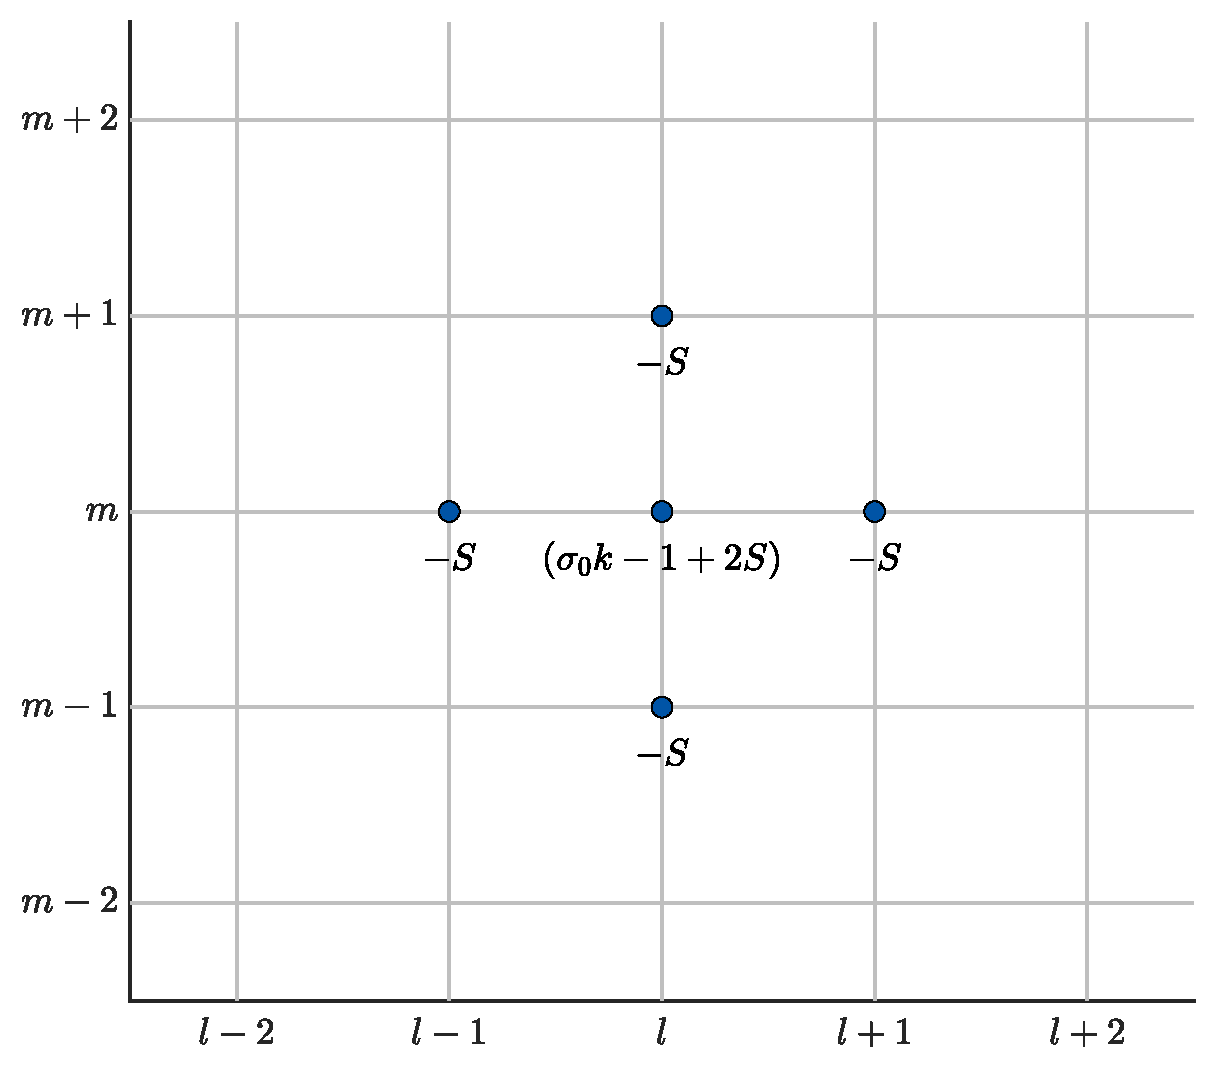
\includegraphics[width=\figWidth]{figures/resonators/2d/prevPlateStencil.eps}}
    \caption{The stencil of the plate with coefficient corresponding to those in update equation \eqref{eq:plateUpdate}. (a) A full overview of the stencil. (b) Stencil of the current time-step $n$. (c) Stencil of the previous time-step $n-1$. \label{fig:plateStencil}}
\end{figure}



\subsection{Frequency Domain Analysis}\label{sec:stabilityThinPlate}
This section follows the process presented in Section \ref{sec:stabilityAnalysis} with the extensions to 2D shown in \ref{sec:stability2Dwave}.

Analysing the compact form of the FD scheme of the thin plate in \eqref{eq:thinPlateFDSCompact} and using Eqs. \eqref{eq:laplacianAnsatz} and \eqref{eq:biharmonicAnsatz} one can obtain a frequency-domain representation of the scheme
and obtain the following characteristic equation
\begin{equation}
    \begin{aligned}
        (1+\sigma_0k)z + &\left(16\mu^2(p_x+p_y)^2 + \frac{8\sigma_1k}{h^2}(p_x+p_y) - 2\right) \\
        &+ \left(1 - \sigma_0k - \frac{8\sigma_1k}{h^2}(p_x+p_y)\right)z^{-1} = 0.
    \end{aligned}
\end{equation}
This can, similarly to the damped stiff string in Section \ref{sec:stiffStringStability}, be solved to
\begin{equation}
    4\mu^2(p_x+p_y)^2 + \frac{4\sigma_1k}{h^2}(p_x+p_y) \leq 1.
\end{equation}
Recalling the definitions $p_x$ and $p_y$ in Eq. \eqref{eq:pxpy}, and given the fact that these are bounded by 1, the following can be written
\begin{gather}
    4\mu^2(1+1)^2 + \frac{4\sigma_1k}{h^2}(1+1) \leq 1\nonumber\\
    16\mu^2 + \frac{8\sigma_1k}{h^2} \leq 1.
\end{gather}
Finally, recalling the definition for $\kappa$ in Eq. \eqref{eq:kappaDef} solving for $h$ then yields
\begin{align}
    &1 \geq \frac{16\kappa^2k^2}{h^4} + \frac{8\sigma_1k}{h^2}\nonumber,\\
    &h^4 - 8\sigma_1kh^2 - 16\kappa^2k^2 \geq 0\nonumber,\\
    &h \geq \sqrt{\frac{8\sigma_1k +\sqrt{(8\sigma_1k)^2 + 64\kappa^2k^2}}{2}}\nonumber,\\
    &h\geq \sqrt{\frac{8\sigma_1k+8\sqrt{\sigma_1^2k^2+\kappa^2k^2}}{2}}\nonumber,\\
    &h \geq 2\sqrt{k\left(\sigma_1 + \sqrt{\sigma_1^2 + \kappa^2}\right)},
\end{align}
which is the stability condition given in Eq. \eqref{eq:stabilityPlate}.

\subsection{Energy Analysis}
Using the steps described in Section \ref{sec:energyAnalysis} with the extensions to 2D presented in Section \ref{sec:energyAnalysis2DWave} one can obtain the total energy of the FD scheme in Eq. \eqref{eq:thinPlateFDSCompact}.
\subsubsection{Step 1: Obtain $\dtp \h$}
To obtain the rate of change of energy, one can take an inner product of the scheme in Eq. \eqref{eq:thinPlateFDSCompact} with $(\dtd \ulmn)$ over discrete (2D) domain $d$ to get
\begin{equation}\label{eq:rOCthinPlate}
    \begin{aligned}
        \dtp \h =&\ \rho H \langle \dtd \ulmn, \dtt \ulmn \rangle_d + D \langle \dtd \ulmn, \dDelta\dDelta \ulmn \rangle_d\\
        & + 2\sz\rho H\langle \dtd \ulmn, \dtd \ulmn \rangle_d - 2\so \rho H\langle \dtd \ulmn, \dtm \dDelta \ulmn \rangle_d = 0.
    \end{aligned}
\end{equation}

\subsubsection{Step 2: Identify energy types and isolate $\dtp$}
Due to the damping present in the system and because the system is distributed in space, the energy balance will be of the following form:
\begin{equation*}
    \dtp \h = \b-\q 
\end{equation*}
where 
\begin{equation}\label{eq:energyBalanceThinPlate}
    \begin{gathered}
        \h = \t + \v, \qwiq \t = \frac{\rho H}{2} \left\lVert\delta_{t-}\ulmn\right\rVert_{d}^2 \quad \text{and} \\
        \v = \frac{D}{2}\langle\delta_{\Delta\boxplus} \ulmn, e_{t-}\delta_{\Delta\boxplus} \ulmn\rangle_{\overline{\underline{d}}}\ .
    \end{gathered}
\end{equation}
and 
\begin{equation}\label{eq:dampingTermThinPlate}
    \mathfrak{q} = 2\sz \rho A \lVert\dtd\ulmn\rVert_d^2 - 2 \so \rho A \langle \dtd \ulmn, \dtm \delta_{\Delta\boxplus}\ulmn \rangle_d.
\end{equation}
The boundary term will not be given here, but can be shown to vanish under 
\subsubsection{Step 3: Check units}
\subsubsection{Step 4: Implementation}



\begin{figure}[h]
    \centering
    \begin{tikzpicture}[->,node distance=3cm,
        thick,main node/.style={circle,draw}]
    
        \node[] (image) at (0,0) {
        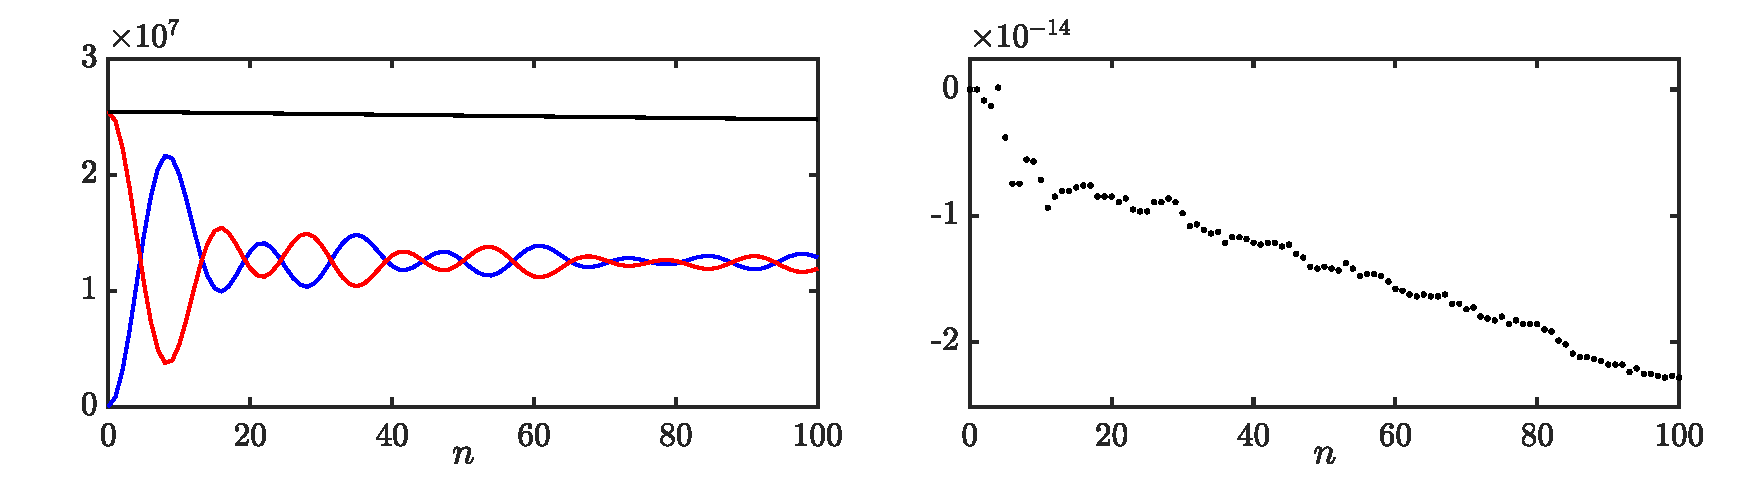
\includegraphics[width=\textwidth]{figures/resonators/2d/energyThinPlate.eps}
        };
    
        \node[] (he) at (0.2,0.5) {\small $\mathfrak{h}_\text{e}$};

        \node[] (h) at (-5.75, 1) {\small $\mathfrak{h}$};
        \node[] (v) at (-5.75, 0.5) {\small $\color{red}\mathfrak{v}$};
        \node[] (t) at (-5.75, 0) {\small $\color{blue}\mathfrak{t}$};
      \end{tikzpicture}
      \caption{The kinetic (blue), potential (red), and total (black) energy of an implementation of the thin plate are plotted in the left panel. Notice that the damping causes $\h$ to decrease. The right panel shows the normalised energy (according to Eq. \eqref{eq:normalisedEnergyDamping}) and shows that the deviation of the energy is within machine precision. \label{fig:energyThinPlate}}
\end{figure}

\section{Stiff membrane}
Like the stiff string, the membrane can be extended with a stiffness term to yield a \textit{stiff membrane} \cite{Fletcher1998}. This model has been used for paper \citeP[F]...
Combining between Eqs. \eqref{eq:2DwavePDE} and \eqref{eq:platePDE} including the losses yields
\begin{equation}\label{eq:stiffMembrane}
    \rho H \ptt u = T\Delta u - D
    \Delta\Delta u
\end{equation}

Is essentially a 2D stiff string. 

\section{Radial Coordinates}\label{sec:radialCoordinates}
This chapter presented various models using a Cartesian coordinate system. Circular or elliptical systems, such as membranes or gongs, could be modelled using a radial coordinate system \cite[Ch. 10]{theBible}. However, using explicit methods to discretise the systems cause the schemes to exhibit high amount much numerical dispersion and reduction of bandwidth \cite[Ch. 11]{theBible}. For better behaviour, one could resort to an implicit scheme, but comes with the drawbacks mentioned in Section \ref{sec:implicitStiffString}. A better alternative is to retain the cartesian coordinate system and set the boundary according to a staircase approximation as done in [\hyperref[ch:listOfPublications]{S4}](see fx. \cite{Hamilton2016, Harrison2018}).